\documentclass[main.tex]{subfiles}

\begin{document}

	\begingroup

	\renewcommand{\cleardoublepage}{}

	\renewcommand{\clearpage}{}

	\chapter{Navigation Function Documentation}

		\chapterauthor{Marc Stelter}
		
		\section{mapping\_hector\_slam}
		It contains a simple launch file starting hector\_slam with the correct parameters for the HSR.
		
		\section{obstacle\_finder.py}\label{met_obstacle_finder}
		Uses the laser scanner in accordance with the map to find objects.
		
		\begin{itemize}
			\item Input: 
				\subitem nav\_msgs/OccupancyGrid
				\subitem sensor\_msgs/LaserScan
			\item Parameter:
				\subitem occ\_threshold 
				Minimum value for a cell in the OccupancyGrid to be occupied
				\subitem min\_scans\_cluster
				Minimum number of laser rays to form a cluster
				\subitem min\_percentage\_covered
				Percentage of a cluster covered by the map to be part of it
				\subitem rad\_neighbor (m)
				Max distance between cells of a cluster
				\subitem error\_map (m)
				Allowed deviation in the map
				\subitem use\_every\_n\_scan
				Skip ecery nth LaserScan message 
			\item  Publish:
				\subitem Topic: /object\_finder
				\subitem Type: geometry\_msgsPoseArray
		\end{itemize}
	
		\begin{figure}[H]
			\centering
			\includegraphics[width=0.7\textwidth]{pictures/obstacle_finder/of_reconfigure.png}
			\caption{Obstacle finder reconfigure}
			\label{img_of_reconfigure}
		\end{figure}
	
		Figure \ref{img_of_reconfigure} shows the reconfigure options for the obstacle finder.
	
		\subsection{How it works}
		
		\subsubsection{Intro}
		
		To better understand how the obstacle finder works it is important to understand how the world is represented in the map. In this case a \href{http://docs.ros.org/kinetic/api/nav_msgs/html/msg/OccupancyGrid.html}{Occupancy Grid} is used.
		
		\begin{figure}[H]
			\centering
			\includegraphics[width=0.7\textwidth]{pictures/obstacle_finder/Gridmap.pdf}
			\caption{Ros Occupancy Grid}
			\label{img_occ_grid}
		\end{figure}
		
		The figure \ref{img_occ_grid} visualizes an Occupancy Grid. For each position in the real world the corresponding x, y index gets calculated based on the resolution. Meaning each cell represents a certain are in the real world. In order to represent negative positions the world position (0,0) is explicitly represented. The values in each cell determine the probability of this cell being occupied. Ranging from 0 (free) to 255 (occupied).
		
		Next it is important to also understand the \href{http://docs.ros.org/melodic/api/sensor_msgs/html/msg/LaserScan.html}{Laser Scan}. 
		\begin{figure}[H]
			\centering
			\includegraphics[width=0.7\textwidth]{pictures/obstacle_finder/laserSnan.pdf}
			\caption{Ros Laser Scan}
			\label{img_laser_scan}
		\end{figure}
		 
		Figure \ref{img_laser_scan} represents the  aspects of the laser scan that are used by the obstacle finder. The scan consists of multiple rays each with their range in m. The min angle is the start angle of the scan. The angle increments represents the angular distance between each scan and the max angle the end angle of the scan.
		
		\subsubsection{Detecting an obstacle}
		
		\begin{figure}[H]
			\centering
			\includegraphics[width=0.7\textwidth]{pictures/obstacle_finder/Cluster-building.pdf}
			\caption{Finding clusters}
			\label{img_finding_cluster}
		\end{figure}   
	
		Figure \ref{img_finding_cluster} is a representation of the occupancy grid with the HSR in it and some exemplary rays of the scanner. In order to find obstacles the rays of a scan get bundled into a cluster. A cluster is a simple Array of the indexes of a ray in the occupancy grid.
		The first step to build clusters from these rays is to determine where the ray ends in the map. This is done by first getting the position of the laser scanner in the map by looking up its transform.
		
		Calculation of the position in the map:\\		
		$range = range of the ray$\\
		$angle = min\_angle + (ray\_index * angle\_increment)$
		
		$x = range * math.cos(angle + scanner.theta) + scanner.x$\\
		$y = range * math.sin(angle + scanner.theta) + scanner.y$\\
		
		Calculation of the indexes in the occupancy grid:\\
		$ix = int((x - origin.x) / resolution)$\\
		$iy = int((y - origin.y) / resolution)$
		
		For the following cluster building only the indexes are considered.
		
		\begin{figure}[H]
			\centering
			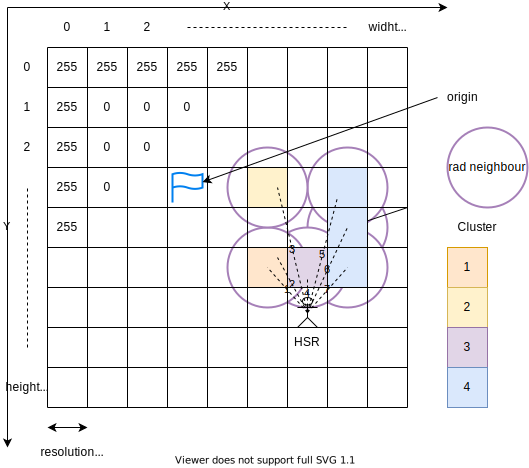
\includegraphics[width=0.9\textwidth]{pictures/obstacle_finder/Cluster-building2.pdf}
			\caption{Finding clusters}
			\label{img_building_cluster}
		\end{figure}
		
		Figure \ref{img_building_cluster} illustrates how the clusters are build. The first ray starts the first cluster. Now the next ray is processed. I is now checked if the rays cell is inside the radius of a cluster. The radius is applied to each cell of the cluster. Since ray 2 and 1 both end in the same cell, ray 2 is added to the cluster. Now ray 3 gets processed. Since the its cell is outside of the radius, it starts a new cluster and replaces the current cluster. Meaning that ray 4 only gets checked against cluster two. Finally the rays 5, 6 and 7 build the last cluster.
		
		\begin{figure}[H]
			\centering
			\includegraphics[width=0.9\textwidth]{pictures/obstacle_finder/Cluster-building3.pdf}
			\caption{Finding clusters}
			\label{img_building_cluster-2}
		\end{figure}
	
		In figure \ref{img_building_cluster-2} the effect of the rad\_neighbour parameter is visualized. Simply by increasing the parameter to also include cells one step away the four clusters become one. This is helpful for very detailed maps with a low resolution where simply checking the neighbor cell may not suffice or if the object is round leading to some of the rays getting lost.
		
		In the next part the found clusters get filtered. The first filter is that a cluster must consist of a minimal amount of rays. This amount is set by the min\_scans\_cluster parameter. Next it is checked whether the cluster is an object or just represent an static obstacle in the occupancy grid.
		
		\begin{figure}[H]
			\centering
			\includegraphics[width=0.9\textwidth]{pictures/obstacle_finder/Cluster-Filter.pdf}
			\caption{Filtering clusters}
			\label{img_filter_cluster}
		\end{figure}
	
		Figure \ref{img_filter_cluster} is based on figure \ref{img_building_cluster} and the clusters have been filtered assuming $min\_scans\_cluster = 2$ has been assumed. Therefore the clusters 2 and 3 have been removed. In addition occupancy values have been added to the grid. Now for each ray of a cluster the corresponding cell in the grid plus all cells inside the radius of the error\_map get checked for their occupancy value. The error\_map parameter has been added to counteract bad localization or maps of poor quality.  Once one of these values is equal or greater than the occ\_threshold parameter the ray counts as matched. Each matched ray get counted and after each ray has been processed the percentage of covered rays is calculated. Should this value be greater or equal than the min\_percentage\_covered parameter the cluster is counted as part of the static map an removed.
		
		For the remaining two clusters in \ref{img_filter_cluster} the result would be the following assuming that:
		\begin{itemize}
			\item occ\_threshold = 40
			\item min\_percentage\_covered = 70\%
		\end{itemize}
	
		\textbf{Cluster 1:}
		Ray 1 and ray 2 match since their cell has a value of 170. Therefore 100\% of the cluster is covered removing the cluster.
		
		\textbf{Cluster 4:}
		Even though the values of the cells for ray 5 and 6 are 0 they both have a cell inside the error radius with a value of 75 marking them as matched. Ray 7 does not match. Therefore 66\% of the cluster is covered letting the cluster pass the filter.
		
		Finally for the remaining clusters the mean position of the rays gets calculated and returned as a \href{http://docs.ros.org/melodic/api/geometry_msgs/html/msg/PoseArray.html}{pose array}. 
		
		\subsection{Example}
		
		\begin{figure}[H]
			\centering
			\includegraphics[width=0.5\textwidth]{pictures/obstacle_finder/scene_gazebo.PNG}
			\includegraphics[width=0.7\textwidth]{pictures/obstacle_finder/result_obstacle_finder.PNG}
			\caption{Result obstacle finder}
			\label{img_res_obs_finder}
		\end{figure}
	
		Figure \ref{img_res_obs_finder} shows a scene in gazebo and the output of the obstacle finder in rviz. The three pringles cans are recognized while the wall is correctly matched.
		
		\section{nav\_fix.py}
		A small node that takes in the original navigation goal and publishes an intermediate goal upon failure. The original goal gets published 3 times.
		
		This small node has proven to be useful inside the HSR lab since some cables seem to be triggering the magnetic sensors.

	\endgroup

\end{document}

